% !TeX root = ../main.tex

\section*{Clustering \footnote{For clustering see section 14 of ``The Elements of Statistical Learning'' (Hastie, Tibshirani, Friedman - 2009). Section 14.3 ``Cluster Analysis'' introduces different flavours of k-means. }}
Grouping or segmenting a collection of objects into subsets or "clusters", such that those within each cluster are more closely related to one another than objects assigned to different clusters. Sometimes the goal also is to arrange the clusters into a natural hirarchy.

All clustering methods attempt to group the objects based on the definition of similarity supplied to it \(\rightarrow\) choice of distance or dissimilarity measure between two objects.

\subsection*{Proximity Matrices}
Sometimes the data is represented directly in terms of the proximity (alikeness or affinity) between pairs of objects. These can either be \textit{similarities} or \textit{dissimilarities}. This type of data can be represented by an \(N \times N\) matrix \(D\), where \(N\) is the number of objects, and each element \(d_{ii'}\) records the proximity between the \(i\)th and \(i'\)th objects.

Most algorithms presume a symmetric matrix of dissimilarities with nonnegative entries and zero diagonal elements. If the original data were collected as similiarities, a suitable monotone-decreasing function can be used to convert them to dissimilarities.

\subsection*{Dissimilarities Based on Attributes}
Most often we have measurements \(x_{ij}\) for \(i = 1, \dots, N\), on variables \(j=1,\dots, p\) (also called \textit{attributes}. We first have to construct pairwise dissimilarities between the observations. In the common case, we define a dissimilarity \(d_j(x_{ij}, x_{i'j})\) (e.g. squared distance \((x_{ij} - x_{i'j})^2\), even though not appropriate for nonquantitive/categorial attributes) between values of the \(j\)th attribute, and then define
\[D(x_i, x_i') = \sum_{j=1}^p d_j(x_{ij}, x_{i'j})\]

\begin{itemize}
    \item Ordinal variables: Convert to numbers on a scale
    \item Categorial(nominal) variables: Dissimialrity has to be described explicitly
\end{itemize}

\subsection*{Object Dissimilarity}
For comparing objects, often a weighted sum of distances is computed:
\[D(x_i, x_i') = \sum_{j=1}^p w_j d_j(x_{ij}, x_{i'j}); \sum_{j=1}^p w_j = 1\]

Note that giving every variable the same weight \(w_j\) doesn't necessarily give all attributes equal influence. The relative influence of the \(j\)th variable is given by \(w_j \cdot \bar{d_j}\), where \(\bar{d_j} = \frac{1}{N^2} \sum_{i=1}^{N}\sum_{j=1}^{N}d_j(x_{ij}, x_{i'j})\) is the average dissimilarity on the \(j\)th attribute. To achieve this the weights have to be set to \(w_j = \frac{1}{\hat{d_j}}\), which doesn't always make sense.

Specifying an appropriate dissimilarity measure is far more important in obtaining success with clustering than choice of clustering algorithm.

\subsection*{Clustering Algorithm}
Three types of clustering algorithms:
\begin{itemize}
    \item \textbf{Combinatorial:} work directly on the observed data with no direct reference to an unterlying probability model.
    \item \textbf{Mixture modeling:} suposes that the data is a sample from some population describe by an probability density function. This density function is characterized by a parameterized model taken to be a mixture of component density functions; each component density describes one of the clusters.
    \item \textbf{Mode seeking("bump hunting"):} take a nonparamteric perspective, attempting to directly estimate distinct modes of the pdf. Observations "closest"to each respective mode then define the individual clusters.
\end{itemize}

\subsection*{Combinatorial Algorithms}
Each observation is uniquely labeled by an integer \(i \in \{1, \dots N\}\). A prespecified number of clusters \(K<N\) is postulated, and each one is labeled by an integer \(k \in \{1, \dots, K\}\). Each observation is assigned to (only) one cluster by an "encoder" \(C(i) = k\), that assigned the \(i\)th observation to the \(k\)th cluster. One seeks the particular encoder \(C^*(i)\) that achieves the required goal, based on the dissimilarities between every pair of observations.

One approach is to directly specify a mathematical loss function and attempt to minimize it through some combinatorial optimization algorithm. Since the goal is to assign close points to the same cluster, a natural loss function would be
$W(C) = \frac{1}{2} \sum_{k=1}^K \sum_{C(i)=k}\sum_{C(i')=k} d(x_i, x_{i'})$ the \textit{within-cluster scatter}.

One can equivalently maximize the \textit{between-cluster scatter} $B(C) = \frac{1}{2} \sum_{k=1}^K \sum_{C(i)=k}\sum_{C(i') \neq k} d(x_i, x_{i'})$

One simple way to solve this is to minimizes \(W\) or maximized \(B\) over all possible assignments of the \(N\) data points to \(K\) clusters. Unfortunally, such optimization by complete enumeration is feasible only for very small data sets.

For this reason, practical clustering algorithms are able to maximize only a very small fraction of all possible encoders \(C\). The goal is to identify a small subset that is likely to contain the optimal one, or at least a good suboptimal partition. Such feasible stratgies are based on iterative greedy descent (initial partition is specified, at each step cluster assignments are changed such that value of criteroen is improved, stop when no more improvement possible).

\subsection*{K-means}
Squared Euclidean distance:
\begin{equation*}
	d(x_i, x_{i'}) = \sum_{j=1}^p (x_{ij} - x_{i'j})^2 = ||x_i - x_{i'}||^2
\end{equation*}

The within-point scatter can be written as
\begin{equation*}
	W(C) = \sum_{k=1}^K N_k \sum_{C(i) = k} ||x_i - \bar{x_k}||^2
\end{equation*}
where \(\hat{x_k}\) is the mean vector associated with the \(k\)th cluster, and \(N_k\) is the number of observations assigned to a cluster. Thus, the critereon is minimized by assigning the \(N\) observations to the \(K\) clusters in such a way that within each cluster the average dissimilarity of the observations from the cluster mean, as defined by the points in that cluster, is minimized.

\textbf{Algorithm:}
\begin{enumerate}
    \item For a given cluster assignment \(C\), compute each clusters mean
    \item Assign each observation to the closest cluster mean
    \item Iterate 1 and 2 until the assignments do not change
\end{enumerate}

Each iteration reduces the value of the critereon, so that convergence is assured, but the solution may be suboptimal. In addition, on should start the algorithm with many different random choices for the starting means, and choose the solution having smallest value of the objective function.

\subsection*{Gaussian Mixtures as Soft K-means Clustering}
The \(K\)-means clustering procedure is closely related to the EM algorithm for estimating a certain Gaussian mixture model. Suppose we specify \(K\) mixture components, each with a Gaussian density having a scalar covariance matrix \(\sigma^2 I\). Then the relative density under each mixture component is a monotone function of the Euclidean distance between the data point and the mixture center. Hence in this setup EM is a "soft" version of \(K\)-means clustering, making probabilistic assignments of points to cluster centers. As the variance \(\sigma^2 \rightarrow 0\), these probabilities become 0 and 1, and the two methods coincide (responsibility of mixture component \(i: \frac{g_i(x)}{\sum_m g_m(x)}\)).

\subsection*{Vector Quantization}
The \(K\)-means clustering algorithm represents a key tool in the apparently unrelated area of image and signal compression, particular in \textit{vector quantization} or \textit{VQ}(Gersho and Gray, 1992).

\textbf{Algorithm}:
\begin{enumerate}
    \item Convert to grayscale
    \item Break image into small blocks, e.g. \(2 \times 2\) blocks of pixels
    \item Each block is regarded as a vector in \(\mathcal{R}^4\)
    \item Apply \(K\)-means
    \item Each of the blocks is approximated by its closest cluster centroid, known as codeword. The clustering process is called the \textit{encoding} step, and the collection of centroids is called the \textit{codebook}.
\end{enumerate}

\subsection*{\(K\)-medioids}
 \(K-\)means stuggels with outliers, because using \textit{squared} Euclidean distance places the highest influence on the larger distances.

 Instead of taking means as cluster center, one can identify the sample inside each cluster, which is nearest to all other samples inside it. One then assigns this sample to be the new cluster center.

 The downside is that \(K\)-medioids is far more computationally intensive.

 \subsection*{Practical Issues}
 In order to use \(K\)-means or -medioids one must select the number of clusters \(K^*\) as initialization. A choice for the number of clusters \(K\) depends on the goal. For data segmentation \(K\) is usually defined a part of the problem.

 Data-based methods for estimating \(K^*\) typically examine the within cluster dissimilarity \(W_k\) as a function of the number of clusters \(K\). Seperate solutions are obtained for \(K \in \{1,2,\dots,K_{max}\}\). The corresponding values generally decrease with increasing \(K\).

\begin{figure}[H]
 	\centering
 	\begin{minipage}[b]{0.49\textwidth}
   	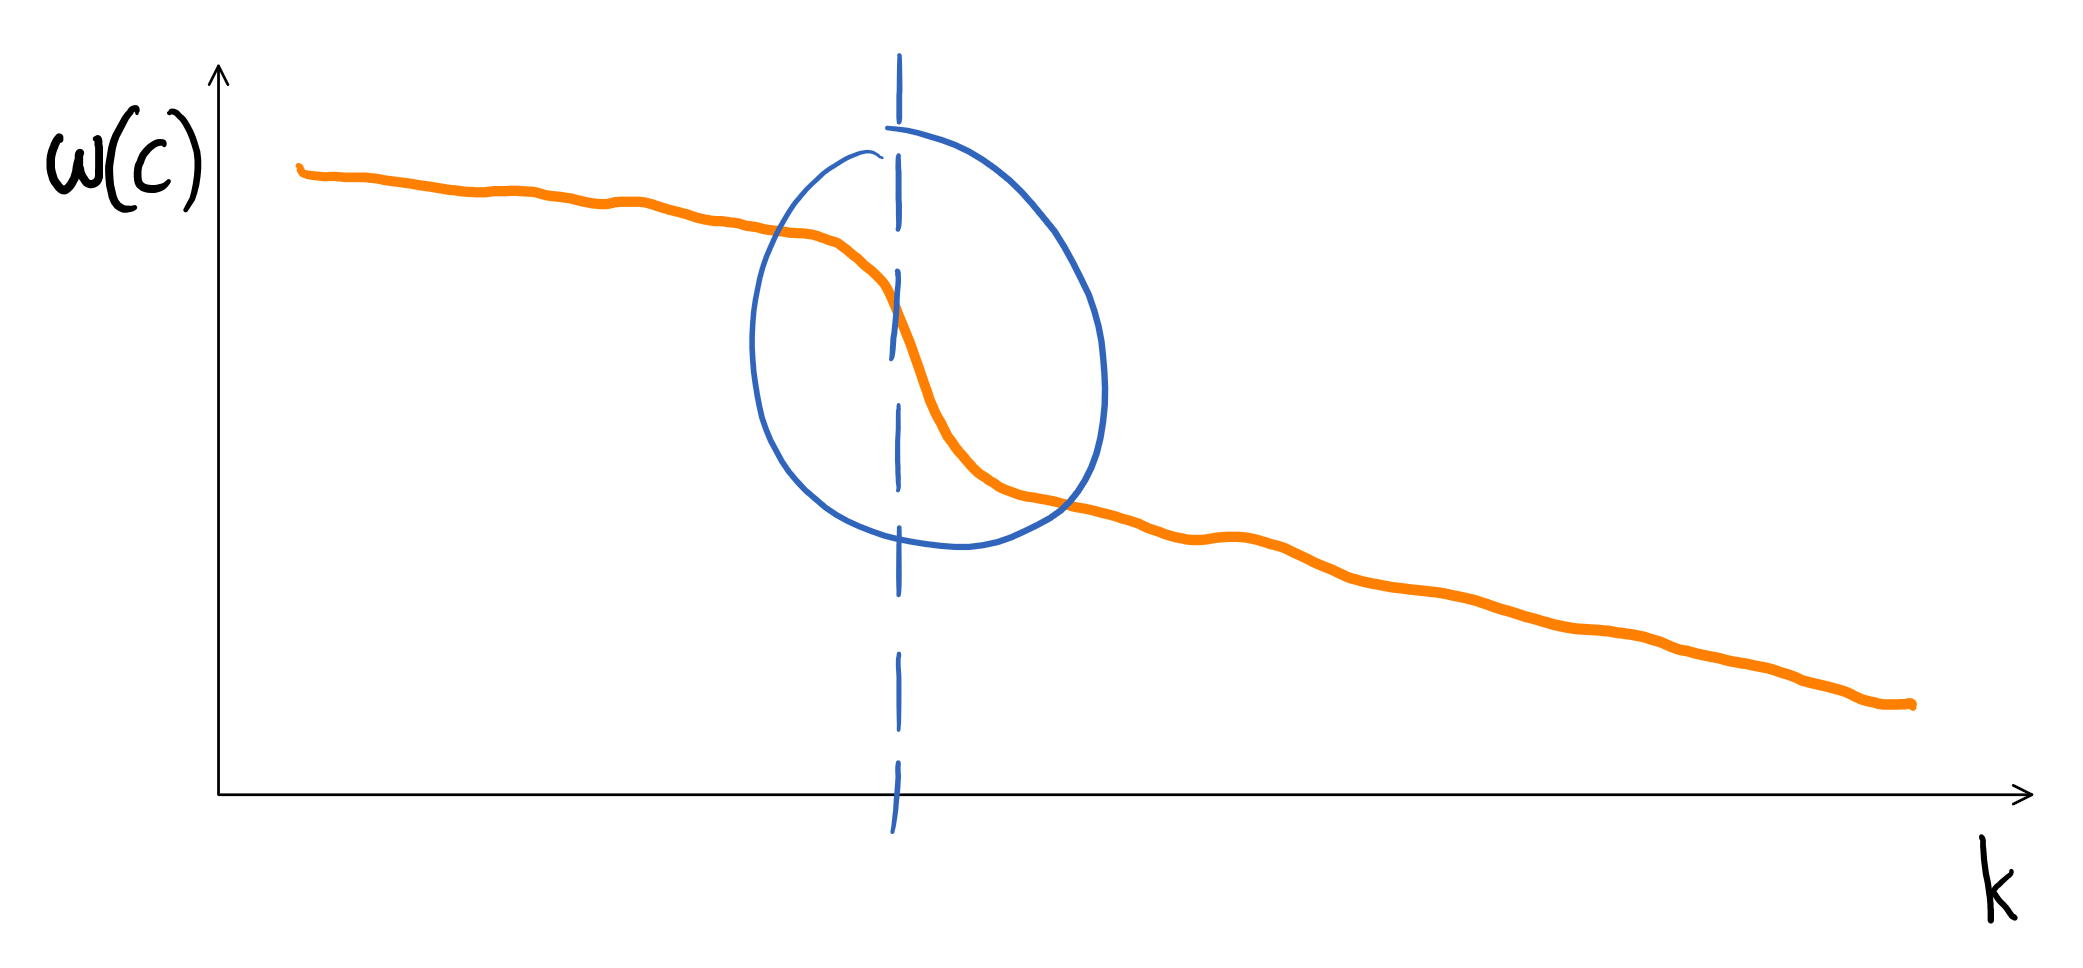
\includegraphics[width=\textwidth]{07-rate-of-change}
   \caption{Approach 1: Track the rate of change of a quality metric (like $w(c)$). Proposed in ``Pattern Classification'' (Duda, Hart, Stork).}
 	\end{minipage}
 	\begin{minipage}[b]{0.49\textwidth}
   	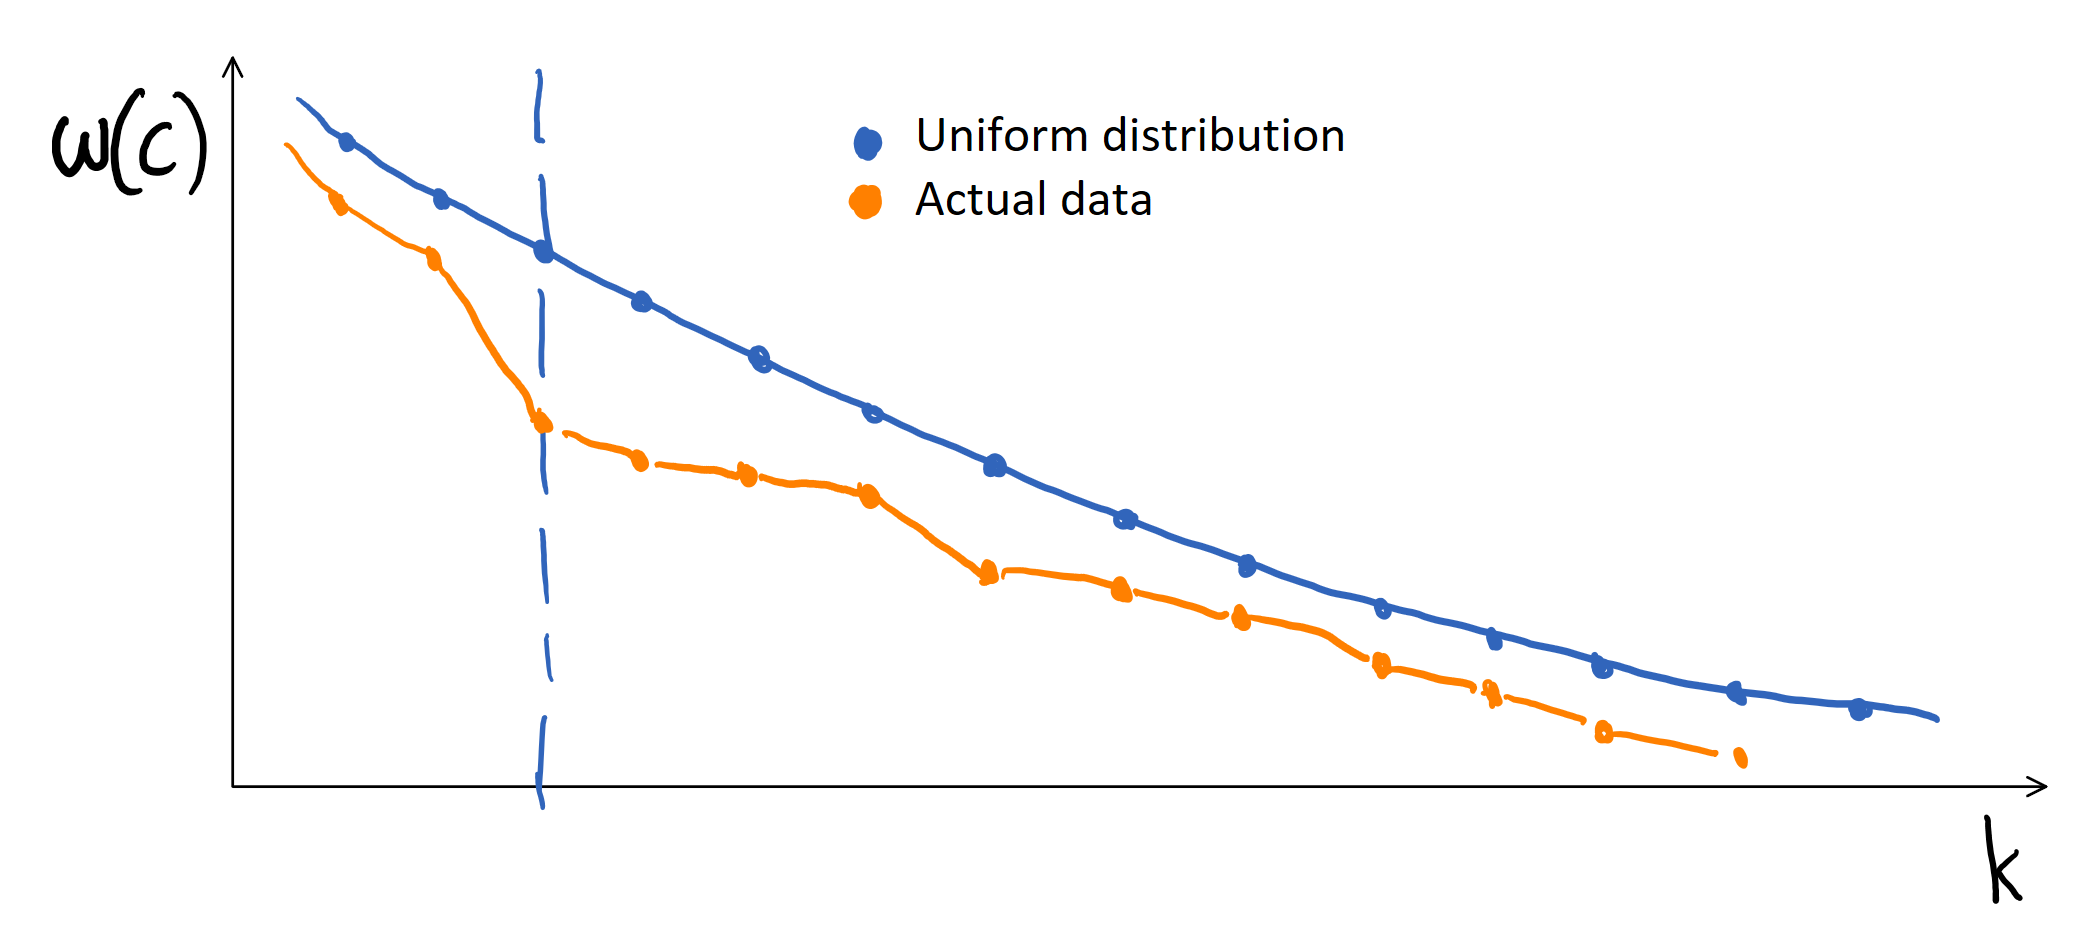
\includegraphics[width=\textwidth]{08-w_c-vs-w_prime_c}
   \caption{Approach 2: Let $w'(c)$ be a metric on a uniform distribution of samples. Relate change of $w(c)$ to change of $w'(c)$. Proposed in TEoSL.}
 	\end{minipage}
\end{figure}

\textbf{Intuition:}
\begin{itemize}
    \item
        \(K < K^*\) will partition actual groups into subsets. The solution criterion value will tend to decrease substantially with each successive increase in the number of specified clusters, \(W_{K+1} \ll W_K\), as the natural groups are successively assigned to seperate clusters.
    \item
        \(K > K^*\) will fuse natural groups into one. This will tend to provide a smaller decrease in the criterion as \(K\) is further increased.
\end{itemize}
\(\Rightarrow\) Splitting a natural group, within which the observations are quite close to each other, reduces the criterion less than partitioning the union of two well-separated groups into their proper constituents.

To the extent this scenario is realized, there will be a sharp decrease in successive differences in critereon value, \(W_K - W_{K+1}\), at \(K=K^*\). An estimate for \(K^*\) is then obtained by identifying a "kink" in the plot of \(W_K\) as a function of \(K\). As with outher aspects of clustering procedures, this approach is somewhat heuristic.

Recently proposed \textit{Gap statistic} (Tibshirani et al., 2001b):
\begin{itemize}
    \item
        Compare the curve \(log W_K\) to the curve obtained from data uniformily distributed over a rectangle containing the data.
    \item
        Optimal \(K\) is where the gap between the two curves is largest
\end{itemize}

\subsection*{Hirarchical Clustering}
Hirarchical clustering methods do not require specifications like for \(K\)-means. Instead, the require the user to specify a measure of dissimilarity between (disjoint) \textit{groups} of observations, based on the pairwise dissimilarities among the observartions in the two groups.

At the lowest level, each cluster contains a single observation. At the highest level there is only one cluster containing all of the data.

Two basic paradigms: \textit{aglomerative} (bottom-up, every step up there is one less cluster) and \textit{devisive} (top-down, every step down there is one new cluster). There are \(N-1\) levels in the hirarchy.

\paragraph{Agglomerative Clustering}
Let \(G, H\) represent two groups. The dissimilarity \(d(G,H)\) is computed from the set of pairwise observation dissimilarities \(d_{ii'}\).\textit{Single linkage} (SL) agglomerative clustering takes the intergroup dissimilarity to be that of the closest (least dissimilar) pair. This is also often called the \textit{nearest-neighbor} technique. \textit{Complete linkage} (CL) agglomerative clustering (\textit{furthest-neighbor} technique) takes the intergroup dissimilarity to be that of the furthest pair. \textit{Group average} (GA) clutering uses the average dissimilarity between the groups (trade-off between compactness/diameter of clusters).

\paragraph{Note:}
We have several options for clustering data. K-means and its variants are straight forward and easy to understand, but if the proper number of clusters is part of the unknowns, it may be a suboptimal choice.
One alternative is mean shift clustering. Here is the number of clusters determined implicitly by the kernel type and size plus the type of bump post process.
